\ofjob{Summoner}
{
	\ofquote{"I don’t like your plan. It sucks."\\}{Yuna}\ofrow
	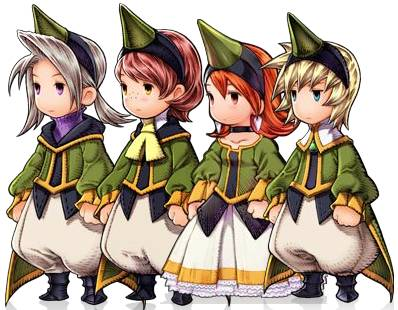
\includegraphics[width=\columnwidth]{./art/jobs/summoner.jpg}\ofrow
	Most powerful heroes are able to call creatures, but the bonds created \accf{Summoners} are far stronger allowing them
	manifest summons for a longer time to fight alongside them on the battlefield.
}
{Rod or Staff}{Robe}{
	Level 1: & HP +16 & MP~+24 & AGI~+2 & STR~+1 \\ 
	Level 2: & HP~+5  & MP~+10 & RES~+1 & MAG~+1 \\ 
	Level 3: & \multicolumn{3}{l}{Archetype Attribute Bonus}   \\
	Level 4: & HP~+5  & MP~+10 & RES~+1 & DEF~+1 \\ 
	Level 5: & HP~+5 & MP~+5  & RES~+2 & MAG~+1 \\  
	Level 6: & HP~+10 & MP~+10 & DEF~+1 \\  
	Level 7: & HP~+5 & MP~+10 & RES~+1 &  MAG~+1      \\  
	Level 8: & HP~+5 & MP~+10 & DEF~+1 &		  \\  
	Level 9: & HP~+10 & MP~+5  & MAG~+1 & RES~+1 \\  
	Level 10: & HP~+10 & MP~+10 & STR~+1 &        	  
}{
	\ofjobspell{Summon}{8}{1r}{1u}{1u}{
		You manifest a creature, that you have the ability to summon, on the battlefield.  
		In combat, summons take their turn right after yours, following your command.
		They are dismissed when they suffer KO, when you summon again or when you dismiss them.
		The HP \& MP of a summon is the same as when it was dismissed, if it suffered KO, it is summoned with 1 HP.
		Summons fully recover their HP \& MP when you go to sleep.
		They level up with you where gain the same attribute increases as you.
		All Summons and the abilities they learn, are shown on the next page.
	}{}{1}\ofabilitygap
	\ofjobpassive{Summon: Carbuncle}{You gain the ability to summon \acc{Carbuncle}.}{1}\ofabilitygap
	\ofjobspell{Image}{6}{0r}{Single}{5u}{The target gains Blink for 3 rounds.}{\blink}{2}\ofabilitygap
	\ofjobspell{Dispel}{10}{0r}{Single}{5u}{All Resiliences and active beneficial Status Effects of the target are removed for 3 rounds.}{}{6}\ofabilitygap
	\ofjobpassive{Summon: Bahamut}{You gain the ability to summon \acc{Bahamut}.}{8}\ofabilitygap
	\ofjobspell{Morph}{24}{1r}{Single}{5u}{The target is turned into a harmless creature of your choice for 3 rounds. In this form he cannot take any action and only move 1u on his turn. Some enemies may be Immune to this effect as decided by the GM. Also, you cannot use this ability consecutively on the same target.
	}{}{10}
}{
	\ofarchetypet{Devout}
	{HP~+7 & MP~+13 & STR~+1 & RES~+2}
	{\ofarchetypespella{Pray}{6}{0r}{1u}{Self}{You and all allies in the target area regain 2d HP.}{}}
	{\ofarchetypepassive{Inferno}{You gain the ability to summon \acc{Ifrit} and permanent Resilience against fire damage. Also, whenever one of your summons deals damage, add your STR and MAG to the summon's for calculating the total damage dealt.}}
	{\ofarchetypereaction{Blood Pact}{Whenever your currently active summon receives any damage, you can redirect half of the total damage dealt to your own HP.}}
	{\ofarchetypespellb{Healing Wind}{14}{0r}{5u (line)}{Self}{You and all allies in the target area regain 4d HP.}{}}
}{
	\ofarchetypet{Evoker}
	{HP~+12 & MP~+8 & MAG~+2 & DEF~+1}
	{\ofarchetypespella{Aero}{6}{0r}{Single}{4u}{You deal 2d wind damage to the target.}{\wind} \ofabilitygap	\ofarchetypespella{Water}{6}{0r}{Single}{4u}{You deal 2d water damage to the target.}{\water}}
	{\ofarchetypepassive{Ice Queen}{You gain the ability to summon \acc{Shiva} and permanent Resilience against ice damage. Also, you can use all spells and techs known by your currently active summon.}}
	{\ofarchetypereaction{Absorb Summon}{Whenever one of your summons suffers KO in combat, you regain an amount of HP and MP equal to 3 times your current Level, as well as EnMAG for 3 rounds.}}
	{\ofarchetypespellb{Aeroga}{14}{1r}{Single}{6u}{You deal 6d wind damage to the target.}{\wind} \ofabilitygap \ofarchetypespellb{Waterga}{14}{1r}{Single}{6u}{You deal 6d water damage to the target.}{\water}}
}
%
\clearpage
%
\ofmonster{Carbuncle}{1}{
\includegraphics[width=0.25\columnwidth]{./art/jobs/carbuncle.png}}
{
	HP: & \hfill 10 & MP: & \hfill 12\\
	STR: & \hfill 1 & DEF: & \hfill 1 \\
	MAG: & \hfill 0 & RES: & \hfill 1 \\
	AGI: & \hfill 3 & Size: & \hfill S\\
}
{\accf{Bite}: 1d DMG (increased to 2d at Level 5)}
{
	\mspell{Thunder \hfill \accf{Level 2}}{4}{0r}{Single}{3u}{You deal 2d lightning damage to the target.}{}
	\mspell{Reflect \hfill \accf{Level 4}}{10}{0r}{Single}{3u}{The target gains a shield that reflects the next spell that targets them back to its caster.}{}
	\mspell{Thundaga \hfill \accf{Level 7}}{12}{1r}{Single}{5u}{You deal 6d lightning damage to the target.}{}
	\mspell{Ruby Light \hfill \accf{Level 8}}{18}{1r}{2u}{5u}{All allies in the target area recover 2d HP and gain a shield that reflects the next spell that targets them back to its caster.}{}
	\mspell{Comet \hfill \accf{Level 10}}{20}{1r}{2u}{5u}{Everyone in the target area makes a DC~8 check and suffers 6d damage upon failure.}{}
}
%
\vspace*{1.8cm}\\
%
\ofmonster{Ifrit}{5}{
\includegraphics[width=0.28\columnwidth]{./art/jobs/ifrit.png}}
{
	HP: & \hfill 32 & MP: & \hfill 24\\
	STR: & \hfill 4 & DEF: & \hfill 2 \\
	MAG: & \hfill 1 & RES: & \hfill 0 \\
	AGI: & \hfill 3 & Size: & \hfill M\\
}
{
	\accf{Claw}: 2d DMG  (increased to 3d at Level 8)\\
	\accf{Resilience}:\fire \hfill \accf{Weakness:}\ice
}
{	
	\mspell{Fire \hfill \accf{Level 5}}{4}{0r}{Single}{3u}{You deal 2d fire damage to the target.}{\fire}	
	\mtech{Burning Strike \hfill \accf{Level 5}}{5}{0r}{Single}{Weapon}{Make an Attack on the target. If you hit, he additionally suffers 2d fire damage.}{}	
	\mtech{Mad Rush \hfill \accf{Level 7}}{8}{0r}{5u (line)}{Self}{You dash forward in an up to 5u long line and deal 4d damage to everyone in the way.}{}	
	\mspell{Firaga \hfill \accf{Level 8}}{12}{1r}{Single}{5u}{You deal 6d fire damage to the target.}{\fire}
	\mtech{Hellfire \hfill \accf{Level 10}}{20}{1r}{2u}{Self}{All enemies in the target area suffer 6d fire damage.}{\fire}	
}
%
\newpage
%
\ofmonster{Bahamut}{9}{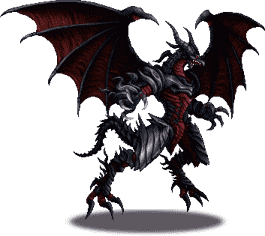
\includegraphics[width=0.3\columnwidth]{./art/jobs/bahamut.png}}
{
	HP: & \hfill 65 & MP: & \hfill 80\\
	STR: & \hfill 6 & DEF: & \hfill 5 \\
	MAG: & \hfill 4 & RES: & \hfill 4 \\
	AGI: & \hfill 3 & Size: & \hfill L\\
}
{
	\accf{Claw}: 3d DMG\\
	\accf{Immune}: All Status Effects \hfill \accf{Resilience:}\dark\fire
}
{
	\mreaction{Final Attack}{If you are about to fall to 0 HP you may use one of your abilities without cost or cast time before falling KO.}
	\mtech{Impulse \hfill \accf{Level 9}}{12}{0r}{3u}{Self}{All enemies in the target area suffer 3d dark damage.}{\dark}{}	
	\mtech{Obliterating Breath \hfill \accf{Level 9}}{14}{0r}{3u (front)}{3u}{Everyone in the target area makes a DC 8 check and suffers 3d damage as well as Poison and Blind for 3 rounds upon failure.}{\poison \blind}{}
	\mspell{Megaflare \hfill \accf{Level 10}}{28}{2r}{2u}{8u}{All enemies within the target area suffer 6d+25 fire damage.}{\fire}
}
%
\vfill
%
\ofmonster{Shiva}{5}{
\includegraphics[width=0.23\columnwidth]{./art/jobs/shiva.png}}
{
	HP: & \hfill 28 & MP: & \hfill 45\\
	STR: & \hfill 2 & DEF: & \hfill 1 \\
	MAG: & \hfill 3 & RES: & \hfill 4 \\
	AGI: & \hfill 2 & Size: & \hfill M\\
}
{
	\accf{Icicle}: 2d DMG, 2u Range  (increased to 3d at Level 8)\\
	\accf{Resilience}:\ice \hspace*{\fill} \accf{Weakness:}\fire
}
{	
	\mspell{Blizzard \hfill \accf{Level 5}}{4}{0r}{Single}{3u}{You deal 2d ice damage to the target.}{}
	\mspell{Deprotect \hfill \accf{Level 5}}{5}{0r}{Single}{5u}{The target suffers DeDEF for 3 rounds.}{\dedef}
	\mspell{Deshell \hfill \accf{Level 5}}{5}{0r}{Single}{5u}{The target suffers DeRES for 3 rounds.}{\deres}
	\mspell{Ice Wall \hfill \accf{Level 7}}{12}{0r}{3u (line)}{5u}{You create a 3u tall and wide wall of ice that blocks the path for 3 rounds. You cannot use this ability again as long as the previous wall still stands.}{}
	\mspell{Blizzaga \hfill \accf{Level 8}}{12}{1r}{Single}{5u}{You deal 6d ice damage to the target.}{\ice}
	\mspell{Diamond Dust \hfill \accf{Level 10}}{20}{0r}{3u (front)}{Self}{All enemies in the target area suffer 6d ice damage. In addition, they make a DC~7 check and suffer Immobile for 1 round upon failure.	}{\ice\immobile}		
}
%
\clearpage